\documentclass[a4paper,12pt]{article}

\usepackage{rotating}
\usepackage[top=1in, bottom=1in, left=0.75in, right=0.75in]{geometry}
\usepackage{graphicx}
\usepackage[numbers,square,sort&compress]{natbib}
\usepackage{setspace}
\usepackage[cdot,mediumqspace,]{SIunits}
\usepackage{caption}
\usepackage{subcaption}
\usepackage{mathtools}
\usepackage{authblk}
\usepackage{float}
\renewcommand{\thesubsection}{\thesection.\alph{subsection}}
\providecommand{\e}[1]{\ensuremath{\times 10^{#1}}}

\begin{document}
\onehalfspacing
\title{PHY 407 Lab 8}
\author{Natalie Price-Jones, 999091021}
\date{31 October 2014}
\affil{\small{natalie.price.jones@mail.utoronto.ca}}
\maketitle

\section{Question 1}

Here, write $\vec{u} = (u,\eta)$

\begin{eqnarray}
\vec{F}(\vec{u}) = \left(g\eta + \frac{u^2}{2}, u(\eta + H)\right)
\label{eqn:vecF}
\end{eqnarray}

\section{Question 2}

\begin{eqnarray}
u_{j}^{n+1} &=& u_j^n - \frac{\Delta t}{2\Delta x}\left(g(\eta_{j+1}^n - \eta_{j-1}^n) + \frac{1}{2}((u_{j+1}^n)^2 - (u_{j-1}^n)^2)\right)\nonumber\\
\eta_{j}^{n+1} &=& \eta_j^n - \frac{\Delta t}{2\Delta x}\left(u_{j+1}^n(\eta_{j+1}^n + H_{j+1}) - u_{j-1}^n(\eta_{j-1}^n + H_{j-1})\right)\nonumber
\end{eqnarray}

\section{Question 3}

\begin{figure}[H]
\centering
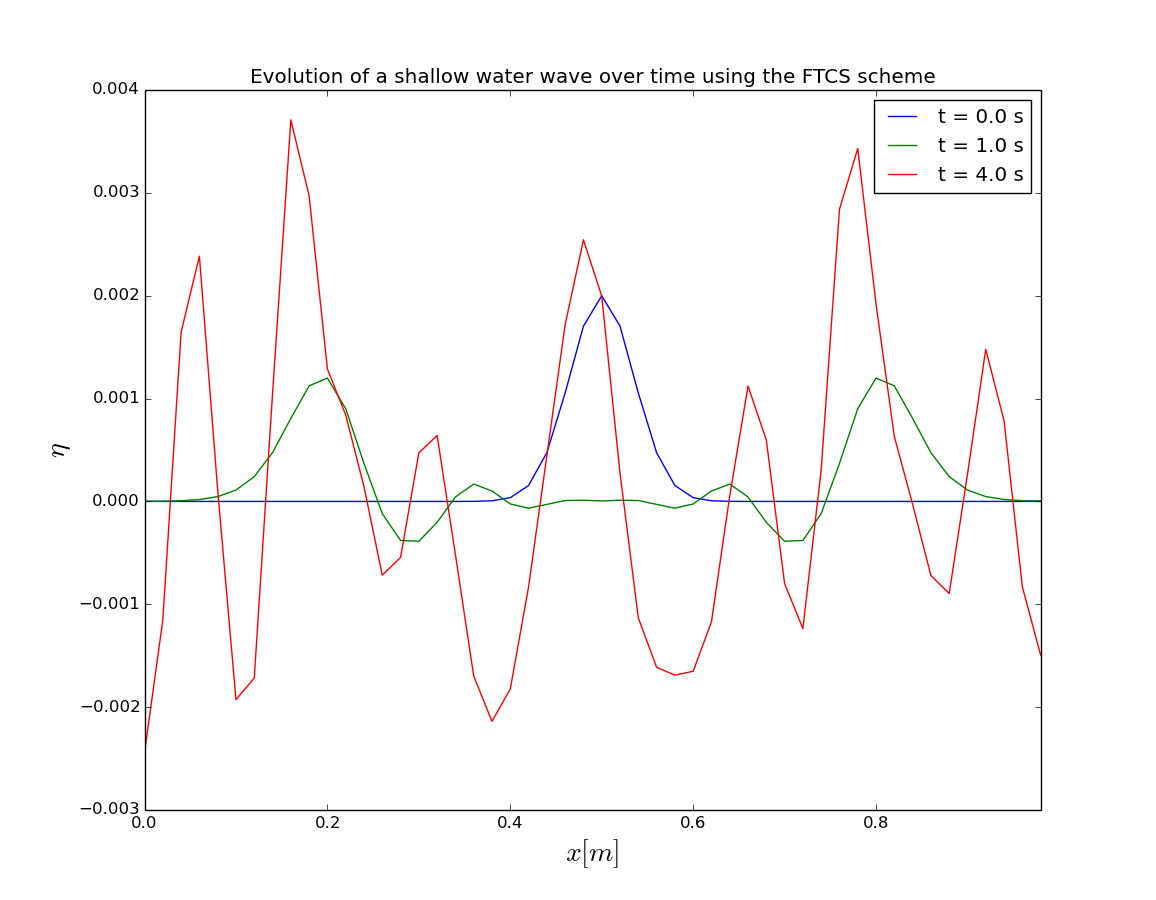
\includegraphics[width = \linewidth]{lab8q3.png}
\caption{}
\label{fig:q3}
\end{figure}

\section{Question 4}

Start by linearizing Equation \ref{eqn:vecF}:

\begin{equation}
\vec{F}(u,\eta) \approx \left(g\eta,uH\right).
\end{equation}

Write $u$ and $\eta$ as Fourier series: 

\begin{eqnarray}
u(x,t) &=& \sum_{k=1}^{\infty}c_k(t) e^{ikx},\nonumber\\
\eta(x,t) &=& \sum_{k=1}^{\infty}d_k(t) e^{ikx}.\nonumber
\end{eqnarray}

We can now approximate our timestepping as follows:

\begin{eqnarray}
u(x,t+\Delta t) &=& \sum_{k=1}^{\infty}c_k(t+\Delta t)e^{ikx}\nonumber\\
&=& \sum_{k=1}^{\infty}c_k(t)e^{ikx} - \frac{\Delta t\,g}{2\Delta x}\left(\sum_{k=1}^{\infty}d_k(t)e^{ik(x+\Delta x)} - \sum_{k=1}^{\infty}d_k(t)e^{ik(x-\Delta x)}\right)\nonumber\\
\eta(x,t+\Delta t) &=& \sum_{k=1}^{\infty}d_k(t+\Delta t)e^{ikx}\nonumber\\
&=& \sum_{k=1}^{\infty}d_k(t)e^{ikx} - \frac{\Delta t\,H}{2\Delta x}\left(\sum_{k=1}^{\infty}c_k(t)e^{ik(x+\Delta x)} - \sum_{k=1}^{\infty}c_k(t)e^{ik(x-\Delta x)}\right)\nonumber\\
\implies c_k(t + \Delta t) &=& c_k(t) - d_k(t)\frac{\Delta t\, g}{2\Delta x}\left(e^{ik\Delta x} - e^{-ik\Delta x}\right),\nonumber\\
d_k(t + \Delta t) &=& d_k(t) - c_k(t)\frac{\Delta t\, H}{2\Delta x}\left(e^{ik\Delta x} - e^{-ik\Delta x}\right)\nonumber
\end{eqnarray}

\[ \vec{c} = (t+\Delta t) = \left( \begin{array}{c}
c_k(t+\Delta t) \\
d_k(t+\Delta t)  \end{array} \right)
= \left( \begin{array}{cc}
1 & -\frac{\Delta t\, g}{\Delta x}\sin(k\Delta x) \\
-\frac{\Delta t\, H}{\Delta x}\sin(k\Delta x) & 1  \end{array} \right) 
\left( \begin{array}{ccc}
c_k(t) \\
d_k(t)  \end{array} \right)\] 

If we call the $2\times 2$ matrix above $\mathbf{A}$, we find the eigenvalues as follows:

\[\mathrm(det)(\mathbf{A}-\lambda \mathbf{I}) = 
\left|\begin{array}{cc}
1-\lambda & -\frac{\Delta t\,g}{\Delta x}\sin(k\Delta x)\\
-\frac{\Delta t\,H}{\Delta x}\sin(k\Delta x) & 1-\lambda
\end{array}\right| = 0\]

We find that the eigenvalues are:

\begin{eqnarray}
\lambda_1 &=& 1 + \sqrt{gH}\left(\frac{\Delta t}{\Delta x}\sin(k\Delta x)\right)\nonumber\\
\lambda_2 &=& 1 - \sqrt{gH}\left(\frac{\Delta t}{\Delta x}\sin(k\Delta x)\right)\nonumber
\end{eqnarray}

For stability, we need $|\lambda| < 1 $. We know that $-1 \leq \sin(x) \leq 1$, so in the the case of $\lambda_1$, we need $\sin(k\Delta x) < 0$. This means we need $\frac{(2n-1)\pi}{k} < \Delta x < \frac{2n\pi}{k}$ ($n$ an integer). In the case of $\lambda_2$, we need $\sin(k\Delta x) > 0$. This means we need $\frac{2n\pi}{k} < \Delta x < \frac{(2n+1)\pi}{k}$ ($n$ an integer). 

Obviously $\Delta x$ cannot simulataneously satisfy both of these conditions, so we expect the FTCS scheme to be unstable for this system (even under a linear approximation).

\section{Question 5}

\begin{figure}[H]
\centering
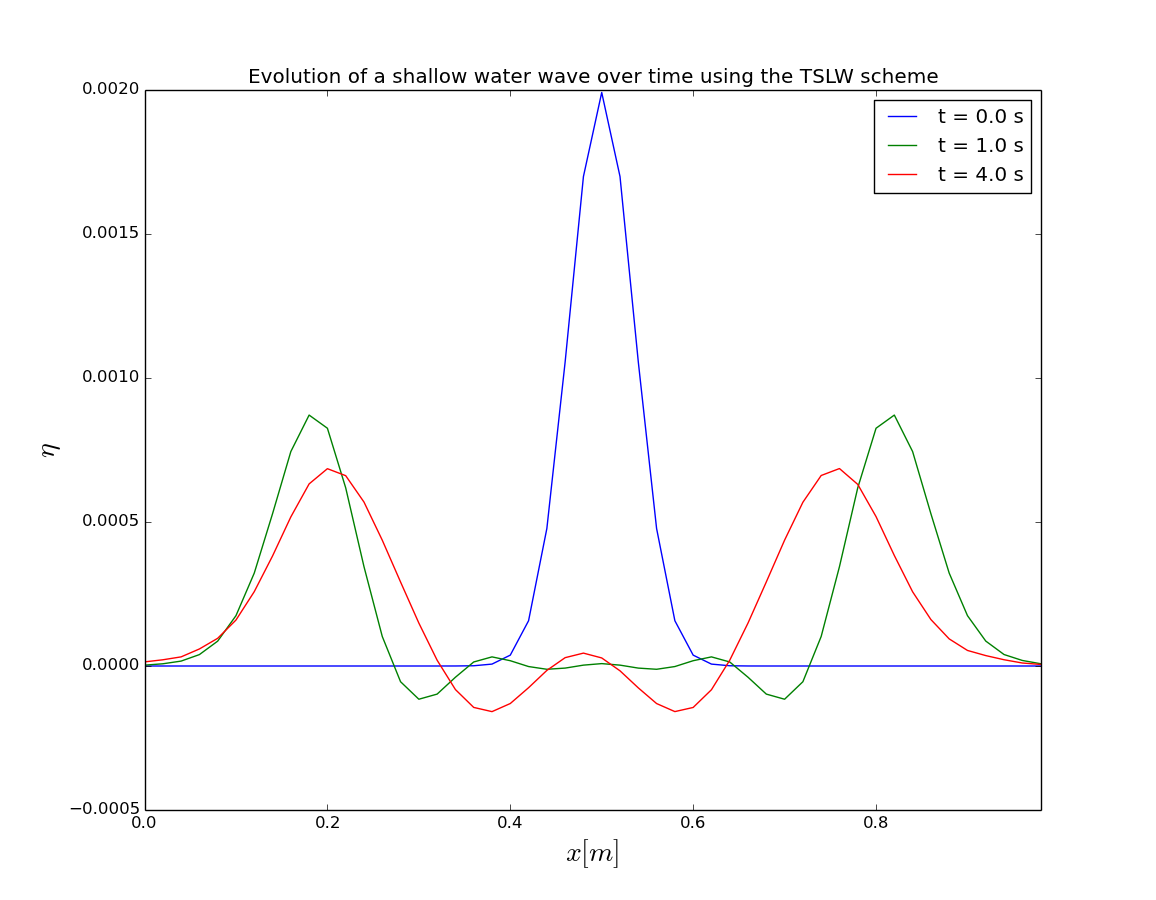
\includegraphics[width = \linewidth]{lab8q5.png}
\caption{}
\label{fig:q5}
\end{figure}

\section{Question 6}

\begin{figure}[H]
\centering
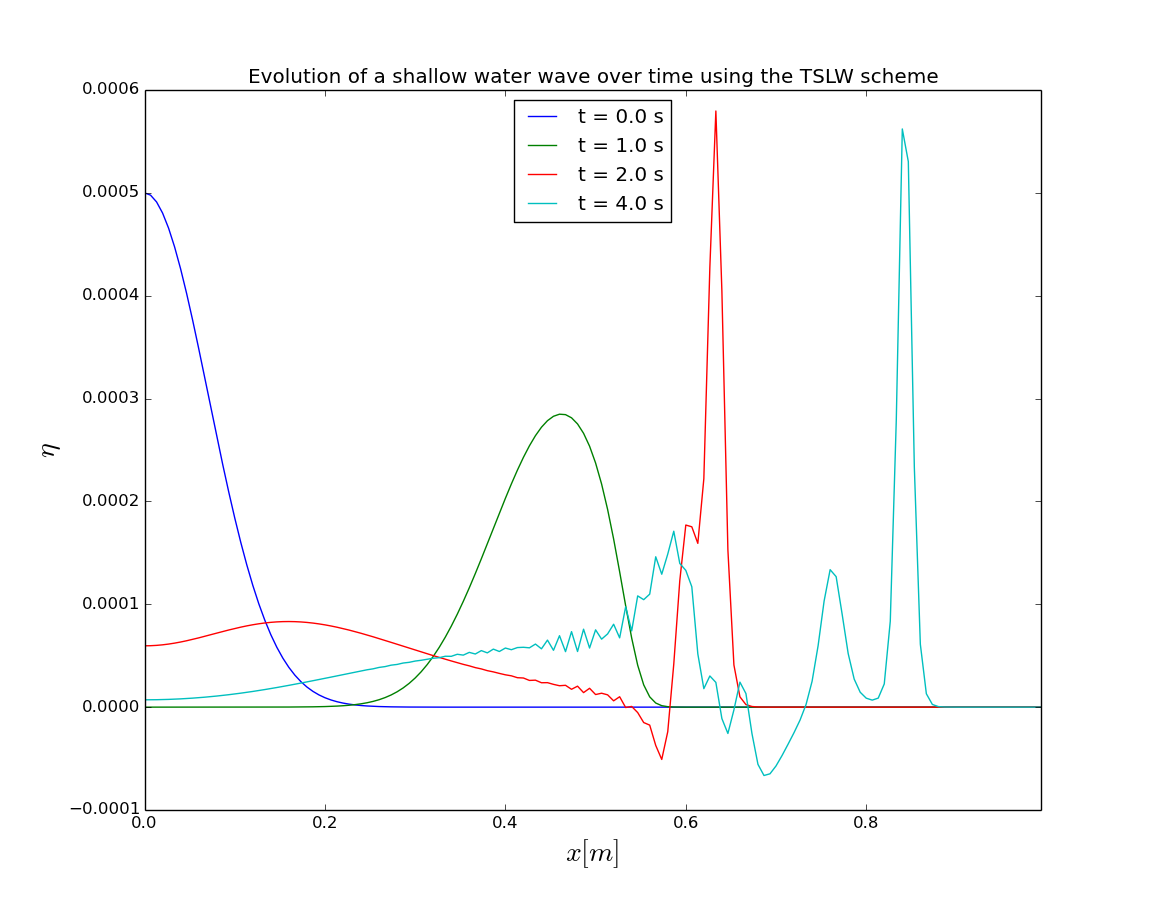
\includegraphics[width = \linewidth]{lab8q6.png}
\caption{}
\label{fig:q6}
\end{figure}

\end{document}